\chapter{Implementación}
\label{implementacion}

\epigraph{Sea lo que sea aquello que cree
o piensa que puede hacer, empiece a hacerlo.
La acción tiene magia, gracia y poder.}%
{\textbf{Goethe}}

El presente capítulo describe algunas características de la puesta a punto de \textbf{Remo}. Se exhibe la representación de datos bioinformáticos, el framework empleado para la distribución de trabajo y algunas porciones de pseudo-código. 

\section{Estructuras y Algoritmos Bioinformáticos}	
\par Ya presentadas las estructuras biológicas básicas en los capítulos anteriores, a continuación se exhibirá la representación de las mismas y algunos algoritmos que son de uso corriente.

\subsection{Representación de nucleótidos, aminoácidos y proteínas}
\par Básicamente, las cadenas de nucleótidos y de aminoácidos que se utilizaron a lo largo de \textbf{Remo} se representaron como cadenas de caracteres (aunque a nivel implementación su representación es mucho más compleja, empleando programación orientado a aspectos mediante templates). Denotamos a las mismas como expresiones regulares, las misma se observan a continuación.
	
\begin{itemize}
	\item $nuc\_dna = a \vert t \vert c \vert g $
	\item $nuc\_rna = a \vert u \vert c \vert g  $	
	\item $aminoacido = Ala \vert Arg \vert Asn \vert ...$	
\end{itemize}
	
\par De la misma forma representamos a los genes de DNA, RNA y proteínas.
		
\begin{itemize}
	\item $gen\_dna = (nuc\_dna)^{+}$	
	\item $gen\_rna = (nuc\_rna)^{+}$	
	\item $proteina = aminoacido (aminoacido)^{+}$
\end{itemize}

\subsubsection{Traducción DNA -$>$ RNA}
\par Existe una forma algorítmica de traducir una secuencia de DNA a una secuencia de RNA (Código 7.1). La misma, consiste en analizar cada nucleótido de la cadena cambiando cada $t$ por $u$.

	\begin{lstlisting}[basicstyle=\tt, frame=trBL, tabsize=4,fontadjust=true]
	gen_rna = traslate(gen_dna), donde: 
		
	gen_rna translate(gen_dna) 
	{
	  forall nuc_dna in gen_dna do 
	  {
	    if nuc_dna is t then 
          replace(nuc_dna, u)
	  }
	}	
	\end{lstlisting}
	\hspace*{3.5cm}\caption{Código 7.1: Traducción DNA -$>$ RNA.}

\subsubsection{Traducción RNA -$>$ proteínas}
\par Podemos traducir la secuencia de RNA (compuesta de nucleótidos) a una secuencia de proteínas (compuesta de aminoácidos). Cabe recordar que cada aminoácido se corresponde por tres nucleótidos (un codón).
\par El algoritmo (Código 7.2) toma cada triplete y lo traduce a un aminoácido correspondiente según la tabla de correspondencia observada en la subsección~\ref{molOrg} (figura~\ref{codGen}).
	
\begin{minipage}{\linewidth}
	\begin{lstlisting}[basicstyle=\tt, frame=trBL, tabsize=4,fontadjust=true]
	protein = translate(gen_rna), donde:
		
	protein translate(gen_rna)
	{
	  i = 0
	  triplet = substr(gen_rna, i, 3)
	  while (triplet != STOP && i < length(gen_rna))
	  {
		aminoacid = genetic_code(triplet)			
		protein += aminoacid
		i += 3						    
	    triplet = substr(gen_rna, i, 3)
	  }
	}
	\end{lstlisting}
\end{minipage}
\hspace*{3.5cm}\caption{Código 7.2: Traducción RNA -$>$ proteínas.}

\section{Decisiones de Implementación}
\subsection{Implementar vs. Integrar}

\par Ante el requerimiento de contar con algoritmos para el cálculo de la estructura secundaria de RNA, se evaluó entre implementar completamente los algoritmos o integrar/adaptar los algoritmos existentes.

\par En este sentido, las interfaces propuestas no descartan ninguna de las dos posibilidades, sino simplemente especifican los ``servicios'' que deben ofrecer al sistema las eventuales implementaciones, ya sean propias o ajenas.

\par Por otro lado, implementar este tipo de algoritmos requiere un profundo conocimiento del dominio (Química Molecular). Además, debido a la complejidad de los mismos, se requieren validaciones empíricas para demostrar la fidelidad de los resultados lo cual excedía el alcance de este trabajo.

\par Finalmente se optó por integrar al sistema los algoritmos para implementar las respectivas interfaces. A continuación se exhibe dicha relación.

\begin{tabbing}
\hspace*{6.5cm} \= \hspace*{5cm} \kill
\hspace*{1cm} \textbf{Interface} \> \textbf{Algortimos} \\
\hspace*{.9cm} fideo::IFold \> UNAFold, RNAFold \\      
\hspace*{1cm}fideo::IHybridize \> RNAup, IntaRNA, RNAcofold, \\
\hspace*{6.6cm}RNAduplex, RNAHybridize \\
\hspace*{1cm}acuoso::ICodonUsageModifier \> GeneDesign \\
\end{tabbing}

\subsection{Método Ad-hoc}
\label{adhoc}
\par En primer instancia, para realizar las comparaciones necesarias de $_m$RNA y $_m$$_i$RNA se empleó un método ad-hoc cumpliendo con los requerimientos definidos\footnote{Visitar el SRS del proyecto para más información: \url{www.r-emo.googlecode.com}}. 
\par Básicamente la idea consistió en fijar cada secuencia de $_m$RNA y por cada secuencia de $_m$$_i$RNA, ir desplazándola de a un nucleótido por vez en el mensajero desde la posición inicial. En cada paso, se realizaron los análisis correspondientes entre nucleótidos.
\par Esta manera de implementar las pasadas de $_m$$_i$RNA sobre los $_m$RNA es ineficiente (Código 7.3). Sin embargo, se escogió adrede esta implementación debido a los siguientes motivos:
\begin{itemize}
	\item Rápido de implementar y testear (*).
	\item Se conocía que el cuello de botella de performance no iba a estar ahí (que tiene O(n$^2$) pero de un N muy chico, 22 nucleótidos aproximadamente que es el tamaño medio de los $_m$$_i$RNA), sino en el folding que es O(n$^3$), con un N dos órdenes de magnitud superior al de las $_m$$_i$RNA.
\end{itemize}

\par (*) Este principio lo cita Donald Knuth\footnote{Donald Ervin Knuth, es uno de los más reconocidos expertos en Ciencias de la Computación por su fructífera investigación dentro del análisis de algoritmos y compiladores. Es Profesor Emérito de la Universidad de Stanford.}, diciendo \emph{``premature optimizations are the mother of all evils''}, lo cual significa que \emph{optimizar antes de tener algo andando, es básicamente la madre de todos los males}.

\par Por otro lado, para que sea O(n), la manera es ir desplazando el $_m$$_i$RNA pero en vez de recorrerlo cada vez que se avanza un nucleótido en el mensajero, solamente sacarle el nucleótido que se descarta, y agregarle el nucleótido que entra. De esta manera, el ciclo completo se hace una sola vez, y luego se opera dos veces por cada desplazamiento (una para el nucleótido que se va y otra para el que entra). Implementarlo de esta manera requería una estructura de todo el programa mucho menos imperativa/secuencial, sino que había que hacer una especie de pipeline como tienen los microprocesadores.

\begin{minipage}{\linewidth}
	\begin{lstlisting}[basicstyle=\tt, frame=trBL, tabsize=4,fontadjust=true]
	try
	{
		Para todo mRNA
		{
			validar secuencia
			obtener mayor seccion codificante
			humanizar mayor seccion codificante
			restablecer secuencia original

			generar archivo de salida
			Para todo miRNA
			{
				obtener nombre de miRNA
				agregar comparaciones al archivo
			}
			restablecer miRNA
		}
	}
	catch (...)
	{
		...
	}
	\end{lstlisting}
\end{minipage}
\hspace*{3cm}\caption{Código 7.3: Pseudo-código $_m$RNA vs. $_m$$_i$RNA.}

\subsection{Formalizando}
\par Luego de analizar los resultados intermedios que se obtuvieron con el método Ad-hoc, se concluyó que el problema es mucho más grande de lo que se pensaba inicialmente, con lo que, nuestra aproximación era demasiada poco precisa, aunque como primer aproximación sirvió. 
%En otros términos, el problema planteado es un problema de mayor envergadura y está resuelto por grandes grupos de investigación que hace muchos años que están en el tema, siempre hablando de interacción $_m$$_i$RNA vs. $_m$RNA, lo cual es sólo una parte del problema, porque dichas investigaciones no tienen en cuenta la \emph{humanización}, que es central en la hipótesis del presente trabajo.
\par Por tal motivo se comenzaron a emplear herramientas más avanzadas, como los son las herramientas de hibridación (subsección~\ref{hibrid}), dado que las mismas cuentan con validaciones empíricas y son confiables.

\section{El Framework FuD}
\par Con el objetivo de distribuir el trabajo en diversos nodos de computación para lograr menores tiempos de espera en los resultado se decidió emplear el framework \textbf{FuD} (del acrónico \emph{FuDePAN ubiquitous Distribution}). \textbf{FuD} es un framework para la distribución de trabajos, o un framework para la implementación de aplicaciones distribuidas\cite{clus09}. Como tal, no depende del problema a implementar y no fuerza ningún modelo de comunicación o disposición de las unidades de procesamiento que serán utilizadas. 
\par En términos generales, \textbf{FuD} se organiza como un esquema \emph{Master-Worker} (un servidor y varios clientes conectados al mismo). Tanto cliente como servidor, se encuentran organizados en tres niveles bien separados (figura~\ref{disenioFud}), cada uno de ellos con una única responsabilidad claramente definida. La comunicación entre los diferentes niveles se encuentra estrictamente limitada, es decir, por cada nivel existe un único punto de comunicación ya sea para comunicarse con la capa superior o con la inferior. Cuando un mensaje es creado, éste debe atravesar las diferentes capas comenzando desde la de nivel más alto hacia la capa inferior, y luego recorrer en sentido contrario las capas del lado. En el apéndice~\ref{detFud} se describen brevemente cada una de las capas que conforman este framework.

\begin{figure}[h!] \hspace{.60cm}
    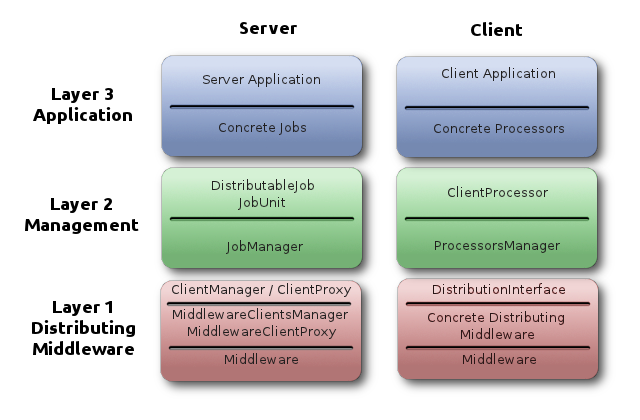
\includegraphics[scale=.55]{image/AbstractLayers.png}
    \caption{Vista abstracta de las capas de \textbf{FuD} [16].} 
    \label{disenioFud}
\end{figure}

\subsection{Conceptos Importantes}
Los siguientes conceptos son necesarios para entender el funcionamiento de una aplicación que usa FuD:
\begin{itemize}
	\item \emph{Cliente:} un cliente es una aplicación conectada al servidor y es el encargado de realizar las tareas de procesamiento.
 	\item \emph{Trabajo:} un trabajo es cualquier tarea a realizar por la aplicación (también llamado trabajo distribuible). Los mismos se
 						  pueden subdividir en unidades de trabajo.
 	\item \emph{Unidad de Trabajo:} representa un cómputo concreto y pertenece a un trabajo particular. No se puede dividir.
 	\item \emph{Manejador de clientes:} módulo encargado de manejar los clientes conectados al servidor.
 	\item \emph{Manejador de trabajos:} módulo de \textbf{FuD} encargado de llevar cuenta de los trabajos (de ambos tipos) que maneja el
 										framework en un momento dado.
 \end{itemize}

\par Como se mencionó anteriormente el cuello de botella en cuanto a complejidad se encontraba en el folding de las secuencias. Las implementaciones del algoritmo de Zuker (UNAFold y RNAFold) no son distribuibles naturalmente, es decir, no se obtiene el mismo resultado al foldear una secuencia completa que al dividirla en tramos, foldear cada uno de los tramos, y unificar los resultados. Por lo cual, el trabajo que se distribuye es el folding de secuencias (original y humanizada), es decir, cada nodo será encargado de foldear cierta secuencia. 
Dado a que \remo necesitaba ser puesto a prueba con un gran número de secuencias para que los resultados sean fiables y consistentes, el uso de \textbf{FuD} benefició notoriamente los tiempo de espera de resultados.

\section{Métricas de Código}
\par Para analizar el código estáticamente se usaron herramientas como CLOC\footnote{http://cloc.sourceforge.net/} (Count Lines of Code) y CCCC\footnote{http://cccc.sourceforge.net/} (\textbf{\textit{C}} and \textbf{\textit{C++}} Code Counter). En esta sección se describen métricas de código generales obtenidas por ambas herramientas y se analizan los resultados obtenidos.

\subsection{Métricas de \textbf{Remo}}
\par \textbf{Remo} esta compuesto por 21 archivos con 3002 líneas de texto a la fecha de publicación del presente documento, dicha cantidad puede variar en el tiempo debido a posibles modificaciones, extensiones o mantenimiento.

\par El cuadro \ref{clocRemo} resume los resultados obtenidos después de correr la herramienta CLOC sobre los archivos de \textbf{Remo}.

\begin{table}[!htf]
    \begin{center}
    \begin{tabular}{|l|r|r|r|r|c|}
    \hline
    \multicolumn{2}{|c|}{Files} & \multicolumn{3}{|c|}{Line Types} & \hspace{0.2cm}\% \\
    \hline
    \textbf{Type} & \textbf{Count} & \textbf{Blank} & \textbf{Comment} & \textbf{Source} & \small{\textbf{\#Comms./Tot.}}\\
    \hline
    \texttt{C++ source} & 10 & 161 & 553 & 1108 & 33.2 \\
    \hline
    \texttt{C++ header} & 11 & 150 & 757 & 273 & 73.4 \\
    \hline
    \textbf{Total}      & 21 & 311 & 1310 & 1381 & 48.6 \\
    \hline
    \end{tabular}
    \caption{Resultados de CLOC para \textbf{Remo} [2].}
    \label{clocRemo}
    \end{center}
\end{table}

\par La herramienta CCCC proporciona un reporte completo sobre las métricas de código, incluyendo métricas de diseño Orientado a Objetos y todo tipo de información relevante en cuanto a código. Un análisis exhaustivo de los resultados de estas métricas se encuentra fuera del alcance del presente trabajo, por lo cual en el cuadro \ref{ccccRemo} se muestra un pequeño resumen de los mismos.

\begin{table}[!htf]
    \begin{center}
	\begin{tabular}{|c|c|c|c|}
	\hline 
	Metric &Tag &Overall &Per Module \\
	 \hline 
	Number of modules &NOM & 31 &  \\
	 \hline 
	Lines of Code &LOC & 342 &11.032 \\
	 \hline 
	McCabe's Cyclomatic Number &MVG & 8 & 0.258 \\
	 \hline 
	Lines of Comment &COM & 787 & 25.387 \\
	 \hline 
	LOC/COM &L\_C & 0.435 &  \\
	 \hline 
	MVG/COM &M\_C & 0.010 &  \\
	 \hline 
	Information Flow measure (  inclusive ) &IF4 & 0 & 0 \\
	 \hline 
	Information Flow measure (  visible ) &IF4v & 0 & 0 \\
	 \hline 
	Information Flow measure (  concrete ) &IF4c & 0 & 0 \\
	 \hline 
	Lines of Code rejected by parser &REJ & 49 &  \\
	 \hline 
	\end{tabular} 
	\caption{Resultados de CCCC para \textbf{Remo} [2].}
	\label{ccccRemo}
\end{center}
\end{table}

\par Para una descripción de Número Ciclomático de McCabe ver ~\cite{McCabe}. 

\subsection{Métricas de Fideo}
\par \textbf{Fideo} esta compuesto por 30 archivos con 3540 líneas de texto a la fecha de publicación del presente documento, dicha cantidad puede variar en el tiempo debido a posibles modificaciones, extensiones o mantenimiento.

\par El cuadro \ref{clocFideo} resume los resultados obtenidos después de correr la herramienta CLOC sobre los archivos de fideo.

\begin{table}[!htf]
    \begin{center}
    \begin{tabular}{|l|r|r|r|r|c|}
    \hline
    \multicolumn{2}{|c|}{Files} & \multicolumn{3}{|c|}{Line Types} & \hspace{0.2cm}\% \\
    \hline
    \textbf{Type} & \textbf{Count} & \textbf{Blank} & \textbf{Comment} & \textbf{Source} & \small{\textbf{\#Comms./Tot.}}\\
    \hline
    \texttt{C++ source} & 10   &    161  &     344   &    967 & 26.2 \\
    \hline
    \texttt{C++ header} & 20   &    243  &    1222   &    603 & 66.9 \\
    \hline
    \textbf{Total}      &  30  &     404 &     1566  &    1570 & 49.9 \\
    \hline
    \end{tabular}
    \caption{Resultados de CLOC para fideo [2].}
    \label{clocFideo}
    \end{center}
\end{table}

\subsection{Métricas de Acuoso}
\par \textbf{Acuoso} esta compuesto por 7 archivos con 663 líneas de texto a la fecha de publicación del presente documento, dicha cantidad puede variar en el tiempo debido a posibles modificaciones, extensiones o mantenimiento.

\par El cuadro \ref{clocAcuoso} resume los resultados obtenidos después de correr la herramienta CLOC sobre los archivos de acuoso.

\begin{table}[!htf]
    \begin{center}
    \begin{tabular}{|l|r|r|r|r|c|}
    \hline
    \multicolumn{2}{|c|}{Files} & \multicolumn{3}{|c|}{Line Types} & \hspace{0.2cm}\% \\
    \hline
    \textbf{Type} & \textbf{Count} & \textbf{Blank} & \textbf{Comment} & \textbf{Source} & \small{\textbf{\#Comms./Tot.}}\\
    \hline
    \texttt{C++ source} & 2 & 26 & 72 & 160 & 31 \\
    \hline
    \texttt{C++ header} & 5 & 46 & 247 & 112 & 68 \\
    \hline
    \textbf{Total}      & 7 & 72 & 319 & 272 & 53 \\
    \hline
    \end{tabular}
    \caption{Resultados de CLOC para acuoso [2].}
    \label{clocAcuoso}
    \end{center}
\end{table}

\subsection{Métricas de Etilico}
\par \textbf{Etilico} esta compuesto por 8 archivos con 624 líneas de texto a la fecha de publicación del presente documento, dicha cantidad puede variar en el tiempo debido a posibles modificaciones, extensiones o mantenimiento.

\par El cuadro \ref{clocEtilico} resume los resultados obtenidos después de correr la herramienta CLOC sobre los archivos de etilico.

\begin{table}[!htf]
    \begin{center}
    \begin{tabular}{|l|r|r|r|r|c|}
    \hline
    \multicolumn{2}{|c|}{Files} & \multicolumn{3}{|c|}{Line Types} & \hspace{0.2cm}\% \\
    \hline
    \textbf{Type} & \textbf{Count} & \textbf{Blank} & \textbf{Comment} & \textbf{Source} & \small{\textbf{\#Comms./Tot.}}\\
    \hline
    \texttt{C++ source} & 2 & 18 & 67 & 145 & 31.6 \\
    \hline
    \texttt{C++ header} & 6 & 64 & 260 & 152 & 63.1 \\
    \hline
    \textbf{Total}      & 8 & 82 & 327 & 297 & 52.4 \\
    \hline
    \end{tabular}
    \caption{Resultados de CLOC para etilico [2].}
    \label{clocEtilico}
    \end{center}
\end{table}

\subsection{Métricas de \textbf{Remo} con Fud}
\subsubsection{Server}
\par \textbf{Remo server} esta compuesto por 8 archivos con 803 líneas de texto a la fecha de publicación del presente documento, dicha cantidad puede variar en el tiempo debido a posibles modificaciones, extensiones o mantenimiento.

\par El cuadro \ref{clocServer} resume los resultados obtenidos después de correr la herramienta CLOC sobre los archivos correspondientes a remo server.

\begin{table}[!htf]
    \begin{tabular}{|l|r|r|r|r|c|}
    \hline
    \multicolumn{2}{|c|}{Files} & \multicolumn{3}{|c|}{Line Types} & \hspace{0.2cm}\% \\
    \hline
    \textbf{Type} & \textbf{Count} & \textbf{Blank} & \textbf{Comment} & \textbf{Source} & \small{\textbf{\#Comms./Tot.}}\\
    \hline
    \texttt{C++ source} & 4 & 59 & 143 & 387 & 0.36 \\
    \hline
    \texttt{C++ header} & 4 & 45 & 129 & 144 & 0.47 \\
    \hline
    \textbf{Total}      & 8 & 104 & 272 & 531 & 0.33 \\
    \hline
    \end{tabular}
    \caption{Resultados de CLOC para remo server [2].}
    \label{clocServer}
\end{table}

\subsubsection{Client}
\par \textbf{Remo client} esta compuesto por 4 archivos con 285 líneas de texto a la fecha de publicación del presente documento, dicha cantidad puede variar en el tiempo debido a posibles modificaciones, extensiones o mantenimiento.

\par El cuadro \ref{clocClient} resume los resultados obtenidos después de correr la herramienta CLOC sobre los archivos correspondientes a un remo client.

\begin{table}[!htf]
    \begin{center}
    \begin{tabular}{|l|r|r|r|r|c|}
    \hline
    \multicolumn{2}{|c|}{Files} & \multicolumn{3}{|c|}{Line Types} & \hspace{0.2cm}\% \\
    \hline
    \textbf{Type} & \textbf{Count} & \textbf{Blank} & \textbf{Comment} & \textbf{Source} & \small{\textbf{\#Comms./Tot.}}\\
    \hline
    \texttt{C++ source} & 2 & 24 & 68 & 94 & 0.41 \\
    \hline
    \texttt{C++ header} & 2 & 21 & 84 & 39 & 0.68 \\
    \hline
    \textbf{Total}      & 4 & 45 & 152 & 133 & 0.46 \\
    \hline
    \end{tabular}
    \caption{Resultados de CLOC para un remo client [2].}
    \label{clocClient}
    \end{center}
\end{table}
\subsection{Análisis de las Métricas}
\par Un dato particularmente interesante sobre los resultados de CLOC, es la cantidad de líneas de comentarios y su porcentaje con respecto al total de líneas de código efectivas. La siguiente fórmula describe la relación comentarios/código y la misma fue usada para calcular la última columna de la tablas exhibidas anteriormente:

$$\frac{\#comment\_lines}{\#comment\_lines + \#code\_lines}$$

\vskip .5cm
\par Este valor ronda aproximadamente el 0.50, lo que significa que hay casi la misma cantidad de líneas de comentarios que líneas de código. Este porcentaje de líneas de comentarios se debe, en mayor medida, a que por cada archivo (por más pequeño que sea) se incluye una cabecera (``header'') definiendo ciertos detalles del archivo tal como se observa en el cuadro~\ref{remoComment}.

\begin{table}[!h]
    \lstset{language=C++}
    \begin{lstlisting}[frame=single]
/**
* @file     CodingSectionObtainer.h
* @brief    CodingSectionObtainer provides the 
*           interface that allows get the coding
*           section of sequence
*
* @author Franco Riberi
* @email  fgriberi AT gmail.com
*
* Contents:  Header file for remo providing class 
*            CodingSectionObtainer.
*
* System:    remo: RNAemo - RNA research project
* Language:  C++
*
* @date      October 2012
*
* This file is part of remo.
*
* Copyright (C) 2012 - Franco Riberi, FuDePAN.
*
* Remo is free software: you can redistribute it and/or 
* modify it under the terms of the GNU General Public 
* License as published by the Free Software Foundation, 
* either version 3 of the License, or (at your option)
* any later version.
*
* Remo is distributed in the hope that it will be useful
* but WITHOUT ANY WARRANTY; without even the implied 
* warranty of MERCHANTABILITY or FITNESS FOR A 
* PARTICULAR PURPOSE. See the GNU General Public 
* License for more details.
*
* You should have received a copy of the GNU General 
* Public License along with Remo. If not, see
* <http://www.gnu.org/licenses/>.
*/
    \end{lstlisting}
    \centering \caption{Comentario Doxygen de encabezado de archivo en \textbf{Remo} [2].}
    \label{remoComment}
\end{table}

\par Para justificar más la alta cantidad de comentarios, todo componente de software, sean estos clases, estructuras, funciones, atributos, etcétera, tiene una descripción detallada a ser interpretada por \textit{Doxygen} (el cuál incluye perfiles de funciones) para la generación de documentación automática. El ejemplo~\ref{remoComment} muestra la notación utilizada para Doxygen exhibiendo además el porqué de la alta tasa de comentarios.

\begin{table}[!h]
    \lstset{language=C++}
    \begin{lstlisting}[frame=single]
/** @brief Get the coding section
*
* Method for obtaining the largest coding section of a 
* given sequence.
* @param src:     original sequence
* @param dest:    larger coding section
* @param posInit: to fill with the starting position 
*                 of the largest coding section
* @return void
*/
void getCodingSection(const biopp::NucSequence& src, 
                      biopp::AminoSequence& dest, 
                      size_t& posInit);
    \end{lstlisting}
    \centering \caption{Comentario Doxygen de una función en \textbf{Remo} [2].}
    \label{remoComment}
\end{table}